\section{Architecture Overview}
The overall system architecture is depicted by Figure \ref{architecture_overview}.

To begin with, the whole system mainly operates within the user Local Area Network. A wireless router is the central point of the entire infrastructure because all the involved devices are connected to it via wireless communication.

The Raspberry Pi board is the backbone of the back-end processing activities. It is in charge of running Node-RED and acts as MQTT broker. It collects information that are sent out by several WiFi-capable modules taking advantage of the publish-subscribe MQTT connectivity protocol. Each module is provided with sensors that gather information about the surrounding environment.

ESP-12E and ESP-32 NodeMCU are the IoT WiFi boards that have been chosen to design the infrastructure. There exists a great variety of sensors that can be hooked up to these ESP modules and ease of programming via Arduino IDE makes them an appropriate choice too. Moreover, they offer full TCP/IP stack support.
Each board does not only publish data, but can also subscribe to a specific topic and receive remote commands to control actuators, such as relays.

The end user is able to visualize a user-friendly, web-accessible dashboard directly from his/her own devices, which must be in the same network of the other system components, in case port forwarding is disabled. The interface is provided by Node-RED development tool.
Furthermore, data are forwarded to ThingSpeak by the Raspberry board in order to log them in a remote database and to enable further analysis: ThingSpeak has integrated support from the numerical computing software MATLAB.

\begin{figure}[H]
	\begin{center}
		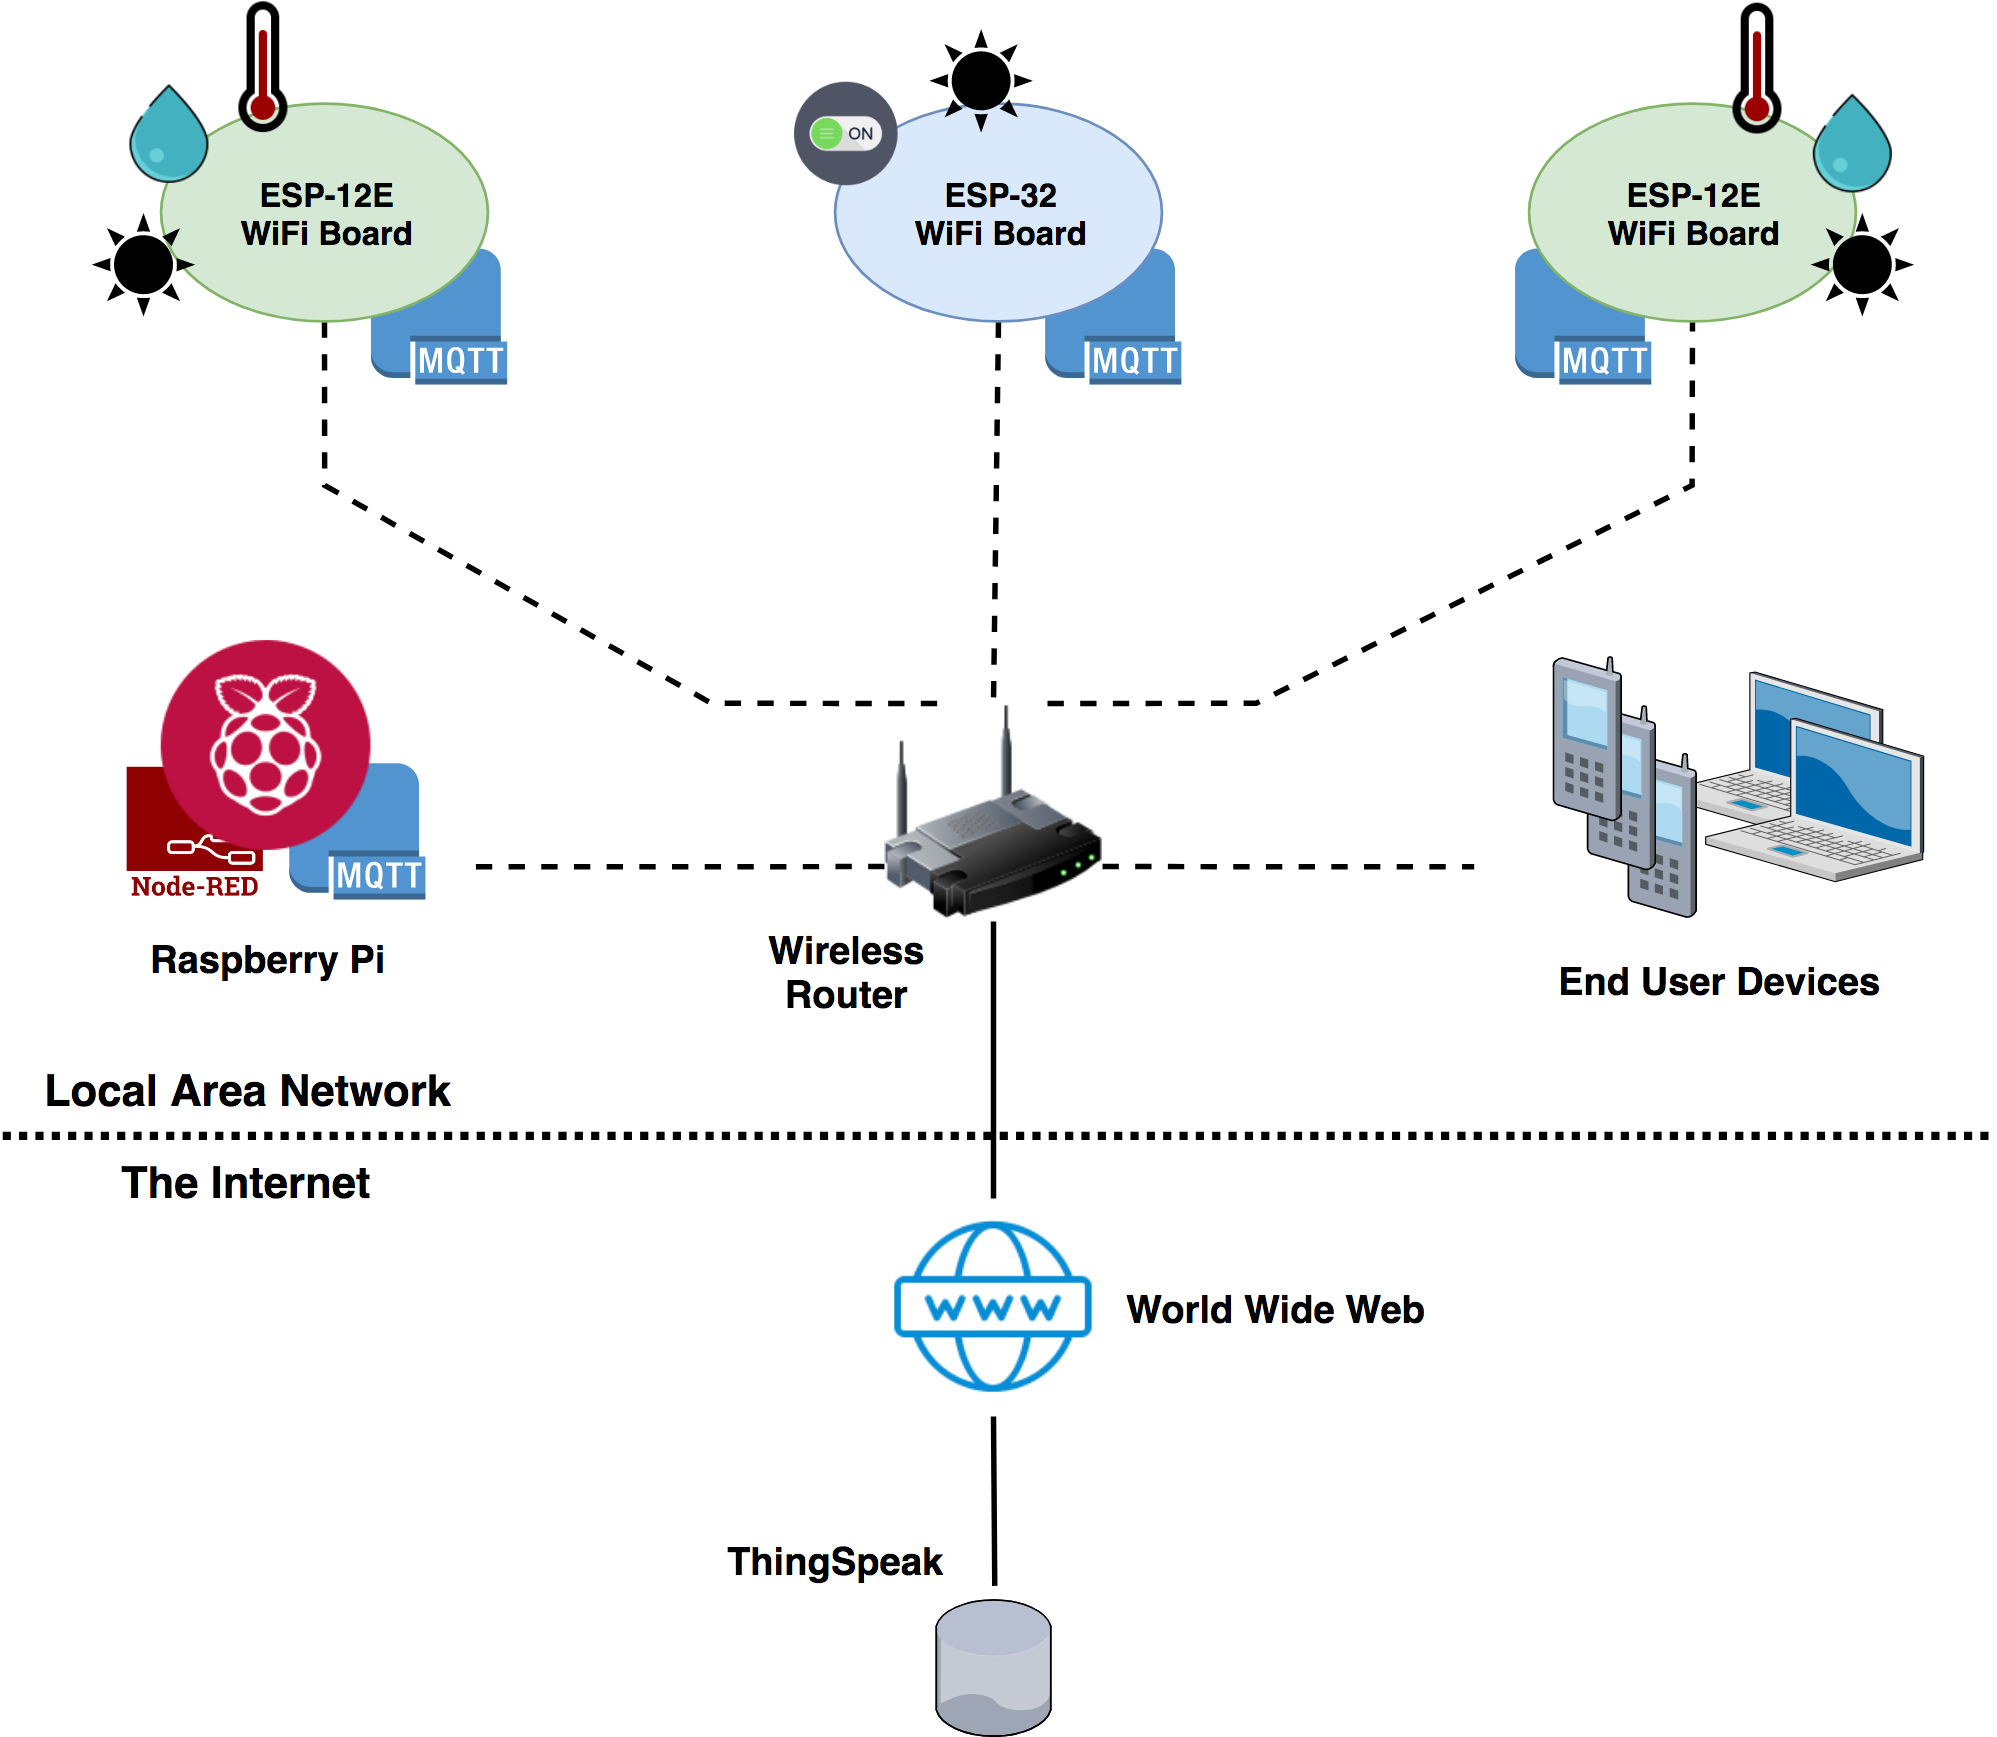
\includegraphics[width=\textwidth]{./pictures/architecture_overview.png}
		\caption{System architecture overview. Dashed lines represent wireless communication, solid lines stand for wired connections.}
		\label{architecture_overview}
	\end{center}
\end{figure}

\section{Configuring the RPi}
The Raspberry Pi is a tiny single-board computer featuring a Broadcom System-On-Chip with an integrated ARM compatible processor. There exist several different generations and models and the role in the system will suit them all. Anyway, using a Pi 3 Model B is highly recommended: it has a quad-core processor and on-board WiFi, Bluetooth and USB boot capabilities which do not require any extra module.

The Raspberry board needs a fresh installation of Raspbian Stretch, the official Debian-based Linux operating system of the Raspberry Pi Foundation. Other third-party operating systems are not taken into account by this document.

\begin{figure}[H]
	\begin{center}
		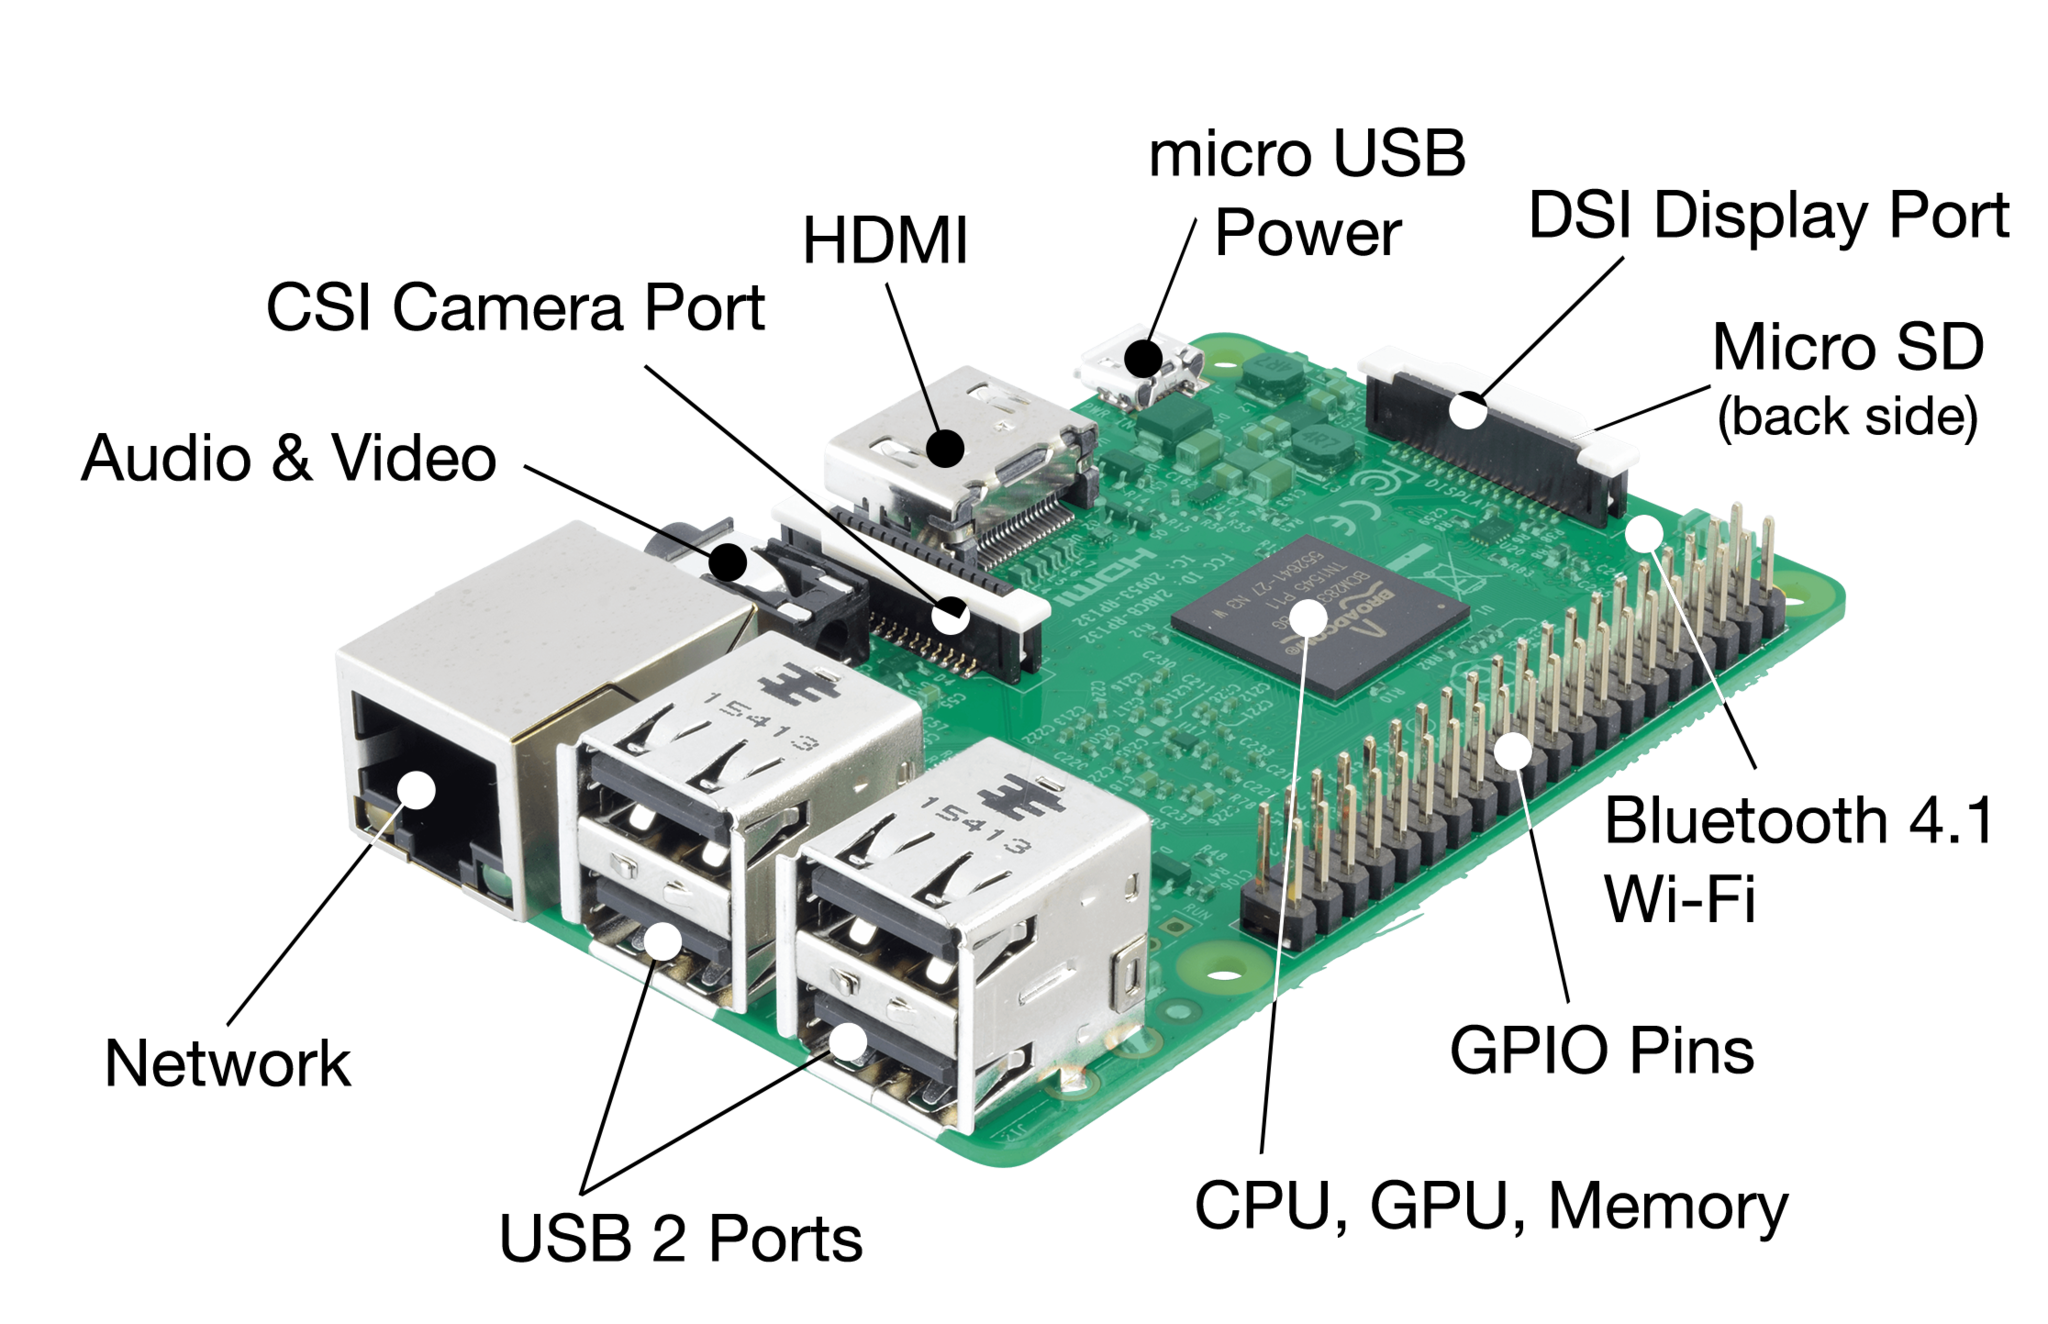
\includegraphics[width=0.6\textwidth]{./pictures/rpi_connections.png}
		\caption{Location of connectors and main Integrated Circuits on the Raspberry Pi 3 Model B.}
		\label{rpi_connections}
	\end{center}
\end{figure}

\noindent
The board is used as headless computer, a device that has been configured to operate without a monitor, keyboard and mouse. The command line is accessed remotely from another computer on the same network using SSH. Since Raspbian has the SSH server disabled by default, it needs to be manually enabled from the desktop or in the terminal via \texttt{raspi-config}.

Setting up a static IP address for the Raspberry is strongly recommended. It can be configured in the DHCP context menu of the wireless router. Since the procedure is different on any device, the handbook should be referred to.

Before proceeding with the following sections, all the software must be up-to-date. This straightforward operation is carried out by executing the commands below in a terminal window:

\begin{verbatim}
    sudo apt-get update
    sudo apt-get upgrade
\end{verbatim}

\subsection{MQTT}
MQTT is a lightweight messaging protocol that works on top of TCP/IP. It provides resource-constrained network clients with a simple way to distribute and exchange information. MQTT is based on the publish-subscribe messaging pattern that requires a message broker to work properly: in this case the role perfectly fits the Raspberry Pi board.

Information about a given topic are sent, or published, to a server that behaves as MQTT message broker. Then, the latter pushes the information out to those clients that have previously subscribed to the above-mentioned topics.

\begin{figure}[H]
	\begin{center}
		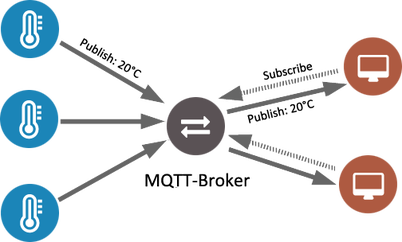
\includegraphics[width=0.6\textwidth]{./pictures/mqtt.png}
		\caption{The message broker is the central point of the MQTT infrastructure. It receives published information and forward it to subscribed clients.}
		\label{mqtt_functioning}
	\end{center}
\end{figure}

\noindent
MQTT offers three quality of service (QoS) levels to guarantee a certain degree of performance to a data flow:

\begin{itemize}
	\item \textbf{0.} At most once delivery: this is the minimal level and guarantees a best effort delivery. A message won't be acknowledged by the receiver or stored by the sender.
	\item \textbf{1.} At least once delivery: all the messages will be delivered at least once to the receiver. This is the QoS level used in the \textit{Home and Automation Monitoring} system because the overhead is lower than QoS 2 and it guarantees the message arrives at least once. Duplicates are not a problem at all because the user interface will be updated one or more time with the same piece of information and this will be completely unnoticeable by the end user.
	\item \textbf{2.} Exactly once delivery. It is the safest and the slowest quality of service level.
\end{itemize}

\subsection{Mosquitto}
Mosquitto is an open source message broker that implements the MQTT protocol. It is suitable for both low-power single board computers and powerful servers.

To install the broker, the following command must be run from the Raspberry Pi terminal:

\begin{verbatim}
    sudo apt-get install mosquitto
\end{verbatim}

\noindent
The broker will automatically start whenever the Raspberry is powered up. The next step is adding users and passwords to secure the MQTT connection. The current directory must be \texttt{/etc/mosquitto} while typing successive commands:

\begin{verbatim}
    // Add the first user
    sudo mosquitto_passwd -c passwordfile user
    
    // Add another user to the existing password file
    sudo mosquitto_passwd -b passwordfile other_user password
\end{verbatim}

\noindent
The following two lines must be added to the \texttt{mosquitto.conf} file.

\begin{verbatim}
    allow_anonymous false
    password_file /etc/mosquitto/passwordfile
\end{verbatim}

\noindent
In this case, just a single user has been created to manage the MQTT connection: username is \texttt{admin} and password is \texttt{hamrpi}. These credentials are used to set up MQTT on both the ESP nodes and Node-RED.

\subsection{Node-RED}
% Cos'è e cosa serve
% Sicurezza con credenziali
% Installazione dashboard
% Blocchi MQTT + credenziali

\section{Getting started with ESP boards}
% Schematici + commento codice
The \textit{Home Automation and Monitoring} system makes use of ESP modules to collect data from sensors and transmit them to the Raspberry Pi taking advantage of MQTT protocol.

Two kinds of boards have been selected to play the role of MQTT client; namely NodeMCU ESP-12E and ESP-32 development kits. The former is based on the widely explored ESP8266 System-On-Chip, which combines WiFi and microcontroller capabilities. The latter utilizes an ESP32 SoC that is very similar, but far more powerful. It has been designed to provide robustness, versatility and reliability in a wide variety of applications.

Both the board can be easily programmed using the Arduino IDE after installing the appropriate cores via Arduino Boards Manager. The core installation will not be covered by this document.

Please notice that there is not a particular reason to use one specific board or the other: they both can fulfill the requirements of the project. The usage of different boards creates heterogeneity and variety, which are always present in the real world. 

\subsection{ESP-12E code and wiring}
An accurate picture of the board pinout is represented by Figure \ref{esp12_pinout}. The ESP8266 module requires 3.3V power supply. Luckily the board provides a voltage regulator and can be connected to 5V using microUSB connector or \textit{Vin} pin.

\begin{figure}[H]
	\begin{center}
		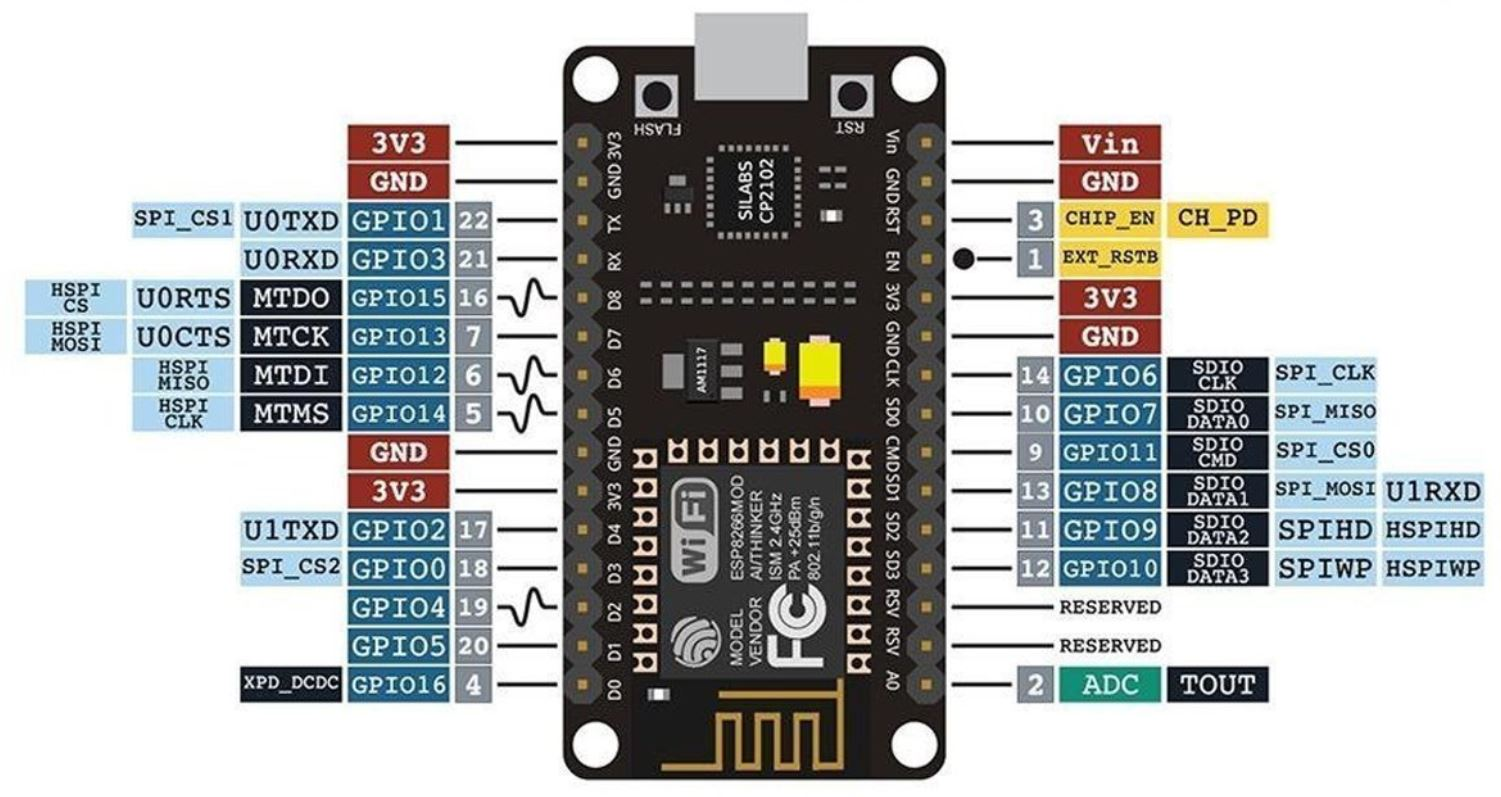
\includegraphics[width=\textwidth]{./pictures/ESP-12E_pinout.JPG}
		\caption{ESP-12E pinout.}
		\label{esp12_pinout}
	\end{center}
\end{figure}

\noindent
There is a number of two ESP-12E boards involved in the project. They both have the same configuration, sensors and wiring. In more details, three LEDs give information about the status of the board:

\begin{itemize}
	\item \textbf{\textcolor{red}{Red}}: the board is trying to get WiFi access.
	\item \textbf{\textcolor[rgb]{1,0.8,0}{Yellow}}: the board is setting up a MQTT connection.
	\item \textbf{\textcolor[rgb]{0,0.6,0}{Green}}: the board is active and it is sending sensor data or listening to subscription messages.
\end{itemize}

% Continuare con schematico e deep sleep

\begin{figure}[H]
	\begin{center}
		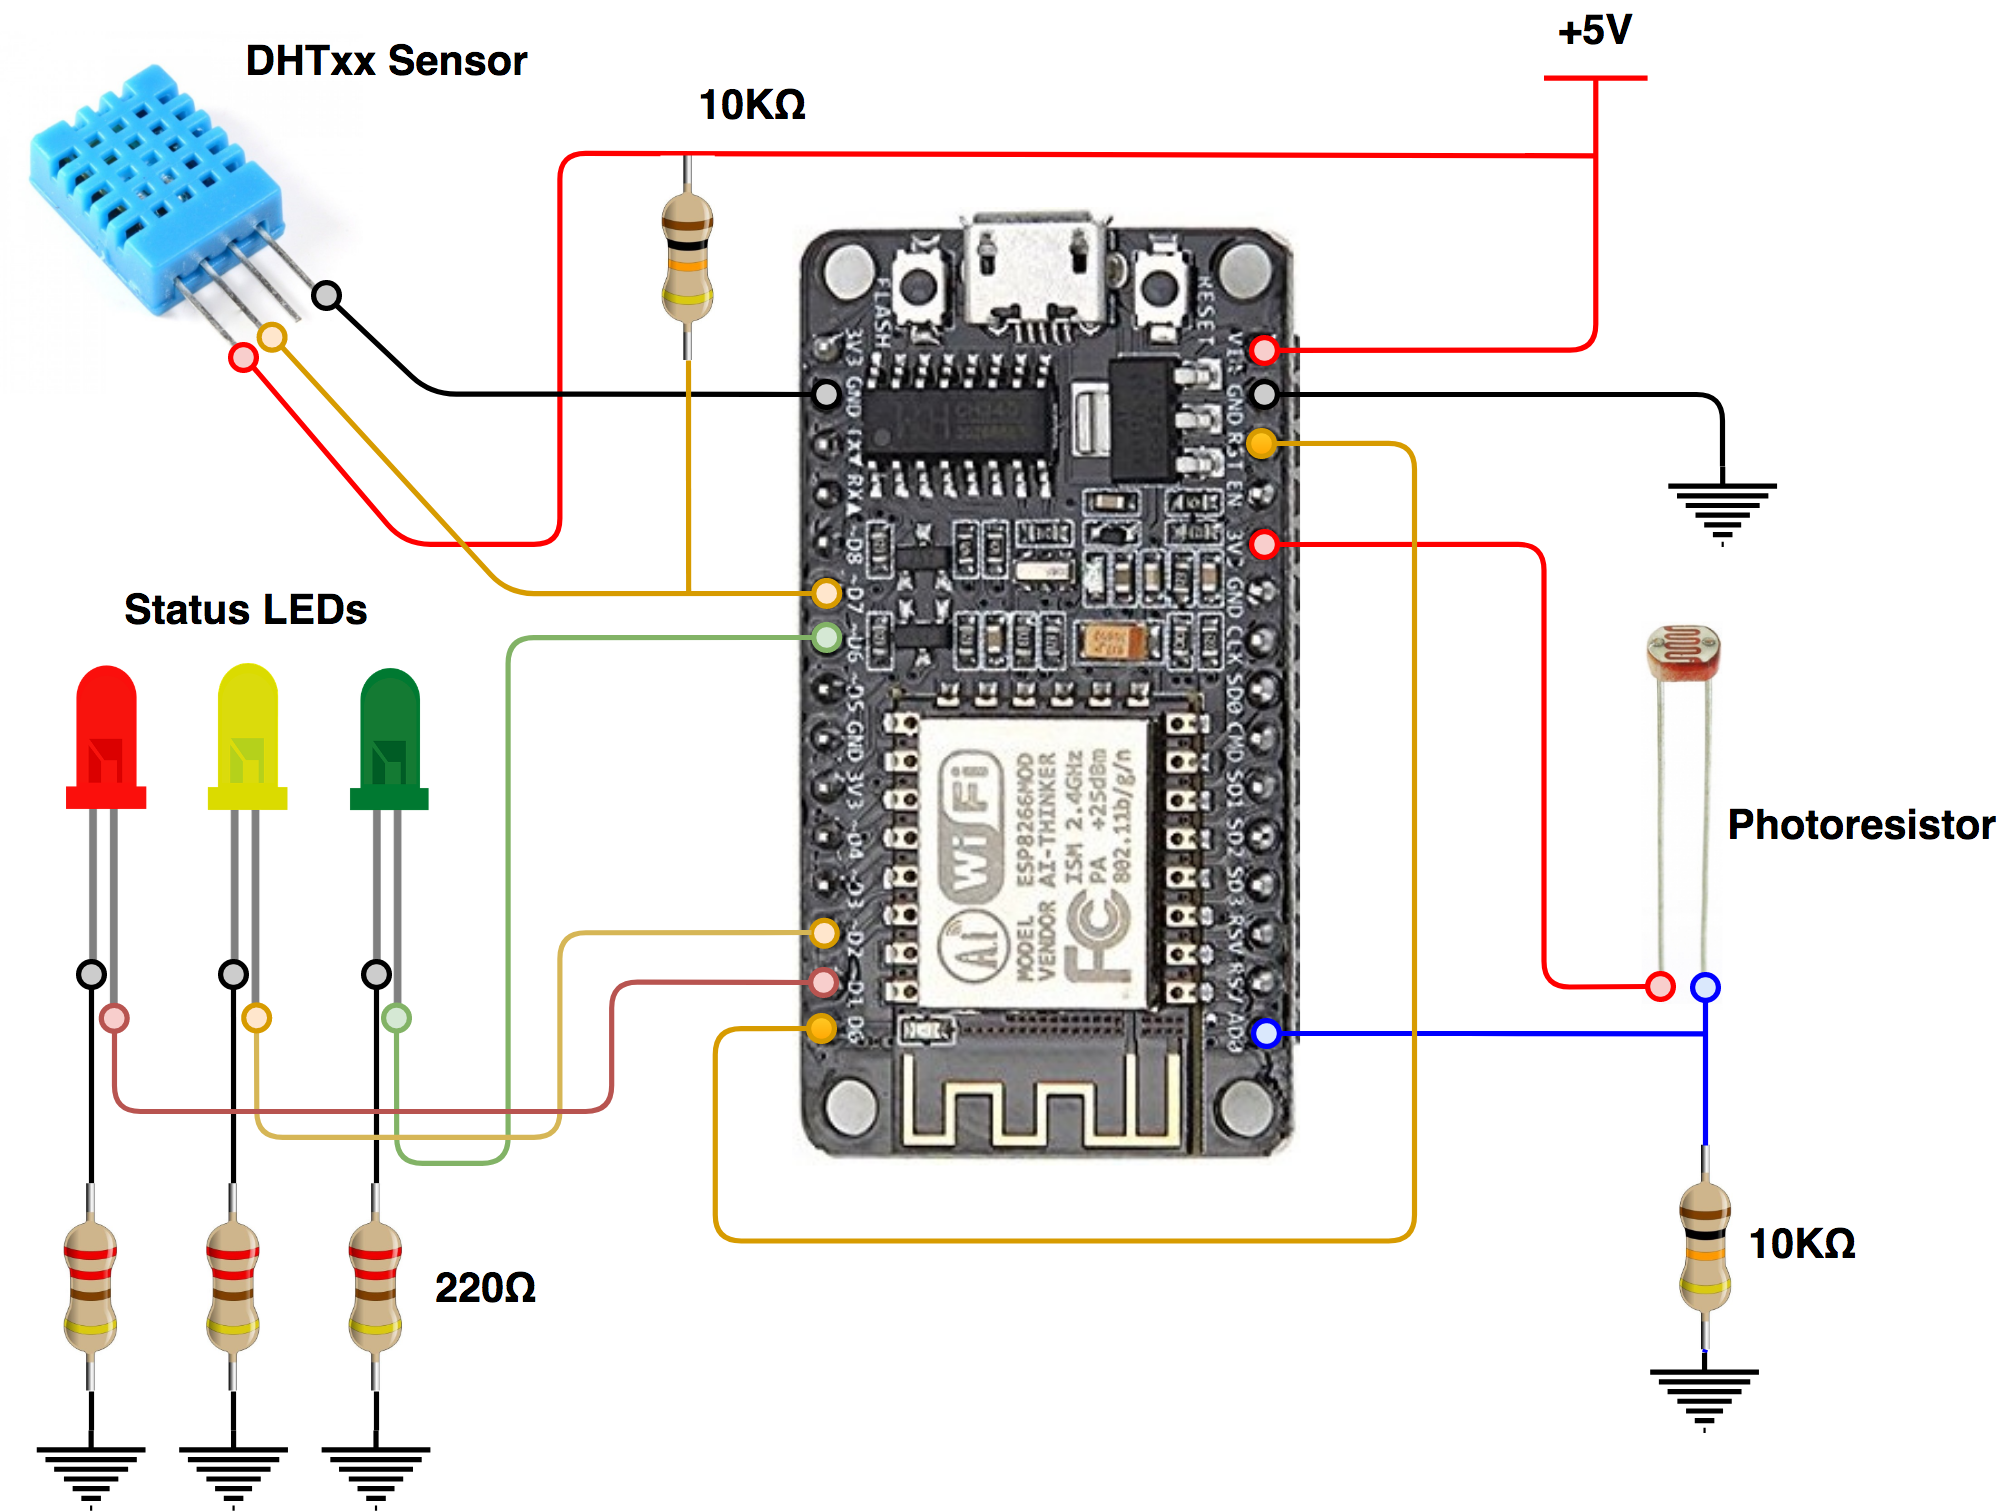
\includegraphics[width=\textwidth]{./pictures/ESP-12E_wiring.png}
		\caption{.}
		\label{esp12_wiring}
	\end{center}
\end{figure}

\section{Connecting to ThingSpeak}
% Cos'è e cosa serve
% Come ci colleghiamo al servizio?
% In breve come si usa